\documentclass[portrait]{sciposter}

\usepackage{amsmath}
\usepackage{amssymb}
\usepackage{multicol}
\usepackage{graphicx}
\usepackage{enumerate}
\usepackage[english]{babel}
\usepackage{fancyvrb}   % for the Verbatim environment
%\usepackage{fancybullets}
%\usepackage{other packages you may want to use}

\usepackage{amsthm}
\usepackage{tikz}
\usepackage{booktabs}
\usepackage{url}

\usepackage{tabularx}
\newcolumntype{R}{>{\raggedleft\arraybackslash}X}

\definecolor{BoxCol}{RGB}{102,153,255}
% uncomment for grey background to \section boxes 
% for use with default option boxedsections

%\definecolor{BoxCol}{rgb}{0.9,0.9,1}
% uncomment for light blue background to \section boxes 
% for use with default option boxedsections

%\definecolor{SectionCol}{rgb}{0,0,0.5}
% uncomment for dark blue \section text 

\newcommand{\bigO}{\mathcal{O}}

\title{\begin{Huge}
A$^*$mbush family: A$^*$ Variations for Ambush 
Behavior and Path Diversity Generation
\end{Huge}}

% Note: only give author names, not institute
\author{Kelwin Fern\'andez, Glebys Gonz\'alez and Carolina Chang}
 
% insert correct institute name
                    
\institute{Universidad Sim\'on Bol\'ivar.
           Caracas, Venezuela}

%\email{kelwin@gia.usb.ve}  % shows author email address below institute

%\date is unused by the current \maketitle

% The following commands can be used to alter the default logo settings
%\leftlogo[0.9]{chenille}{  % defines logo to left of title (with scale factor)
%\rightlogo[0.52]{otherlogo}  % same but on right
% NOTE: the logo image files chenille.png, resp. otherlogo.png must be 
%       present in the same directory as this LaTeX source, either
%       in the .png format, or in any other supported format
%%%%%%%%%%%%%%%%%%%%%%%%%%%%%%%%%%%%%%%%%%%%%%%%%%%%%%%%%%%%%%%%%%%%%%%%%%

\begin{document}
%*** print the poster header defined above: title, authors, affiliations:
\maketitle

%*** facultative: where the poster was presented (appears as a left footer):
\conference{Motion in Games, Rennes, France, November, 2012}

\begin{multicols}{2}
\section*{\large{Motivation}}
\begin{large}
\begin{itemize}
\item Generating agents with \textbf{intelligent-looking} behaviors
has been a constant challenge in the area of Artificial
Intelligence for video games. The user expects to see
agents that can perform \textbf{tactical movements} and
\textbf{group strategies}.

%\item These behaviors tend to be complex in their implementation
%and usually result in pre-established moves that can be easily
%identified by the user.

\item 
A situation that appears frecuently in this area 
is having a group of agennts trying to reach 
 a common target  through pathfinding.
The goal point is usually given by a location in the game map
(potentially the opponent's position).

\item A well known approach is to generate the \textbf{minimal path}
towards the objective.
When the algorithm is executed independently by multiple agents,
it is very likely for the paths to be \textbf{confluent}. Thus,
route diversity and map exploration is prevented.

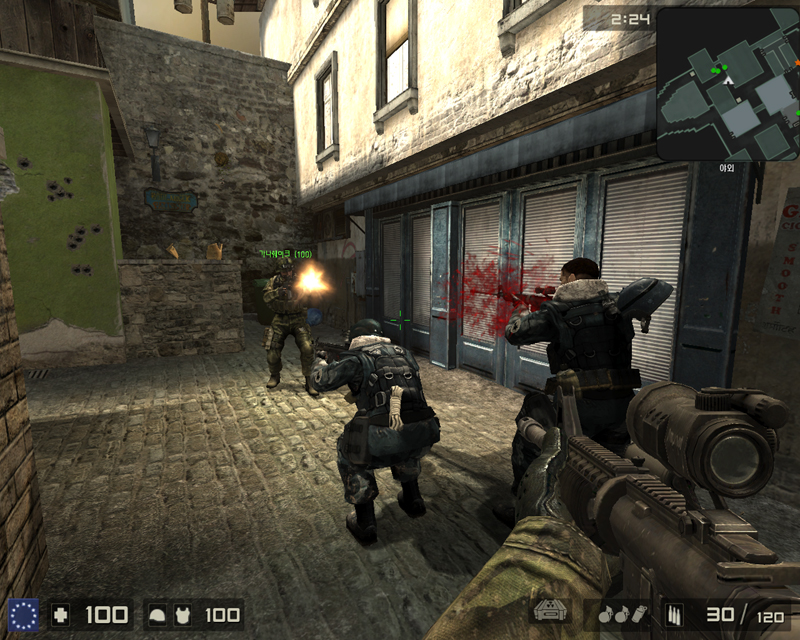
\includegraphics[width=0.15\textwidth, height=10cm]{figures/fps.jpg}
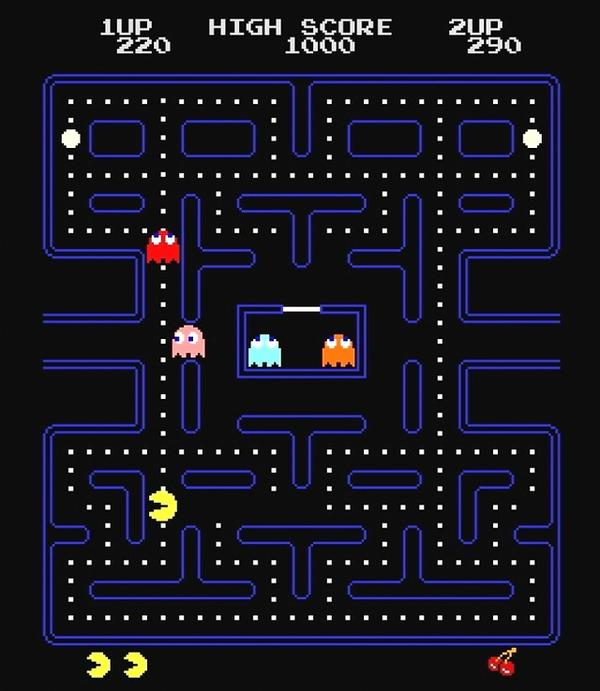
\includegraphics[width=0.15\textwidth, height=10cm]{figures/pacman.jpg}
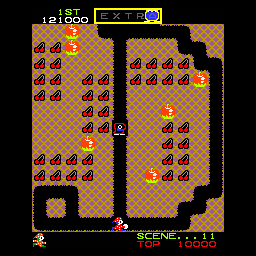
\includegraphics[width=0.15\textwidth, height=10cm]{figures/do.png}

\bigskip
\item When the minimal path strategy is applied for chasing
the enemy, many escape paths are left open. Therefore,
it is of special interest to generate mechanisms of \textbf{route
diversification} that can produce ambush behaviors.
\end{itemize}
\end{large}

\end{multicols}

\section*{A$^*$mbush: The Initial Variation}

\begin{multicols}{3}
\begin{minipage}{0.3\textwidth}

\section*{Formal Problem Definition}
\begin{itemize}
\item Let $G = (V,E)$ be a \textbf{graph} (directed or undirected).

\item Let $A$ be a \textbf{set of agents} that want to reach a point
$t \in V$. Every agent $i \in A$, is located in a node of the
graph. Let $pos(i)$ be the position of the agent $i$.

\item A function over $i$ is defined for  determining the
\textbf{cost} of the displacement of the agents  through the graph
$\lambda_i : E \longrightarrow \mathbb{R}^{\geq 0}$.

\item Let $path(i)$ having $i \in A$, be the \textbf{path} that the 
agent $i$ is taking to reach node $t$.

\item The \textbf{degree of ambush} towards the node $t$ is defined as:\\

$\Phi(t) = \dfrac{|\{ i : path(j) = <pos(j),\ \ldots,\ i,\ t>, j \in A\}|}
{\min(|\{ <i,t> : <i,t> \in E \} |,|A|) }$

\end{itemize}
\end{minipage}
\section{A\*}
\begin{minipage}{0.3\textwidth}
\section*{A*mbush}

\begin{itemize}

\item A$^*$mbush is an $A^*$-based algorithm that solves the
ambush generation problem. 

\item It consists of a \textbf{modification} of the $g$ function,
that favours path diversity. We will call this function $g'$.

\item Let $\Psi(v,i) = 1+(\# j : j \in A \wedge v \in path(j))$,
be the number of agents different from agent $i$, that have the 
node $v$ in their paths towards $t$ plus one.

\item $g'(pos(i),i) = 0$ for the initial node.

\item $g'(w, i) = g'(v,i) + \lambda_i(<v,w>) \cdot \Psi(w,i)^2$
for every expanded edge $<v,w>$.

\item The properties of $A^*$ are preserved. Nevertheless, the path
\textbf{might not be optimal} for the original costs function $g$.

\end{itemize}

\end{minipage}
\end{multicols}

\bigskip
\begin{center}
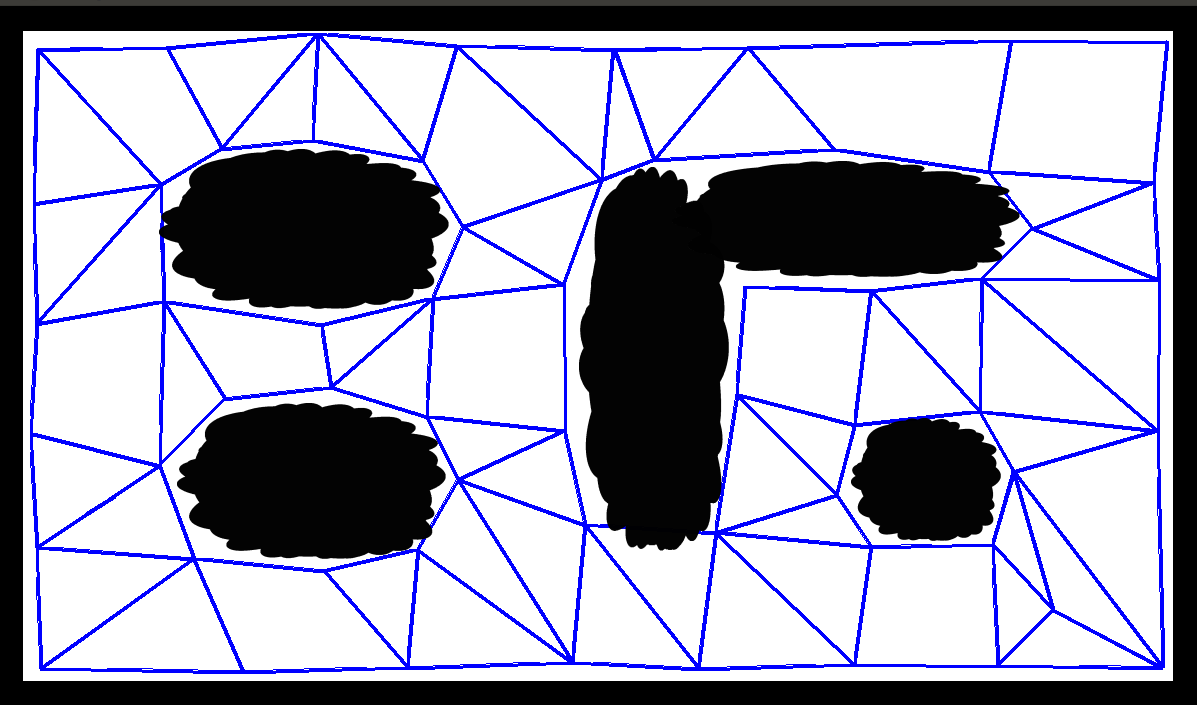
\includegraphics[width=0.25\textwidth]{figures/g2.png}
\hspace*{0.25cm}
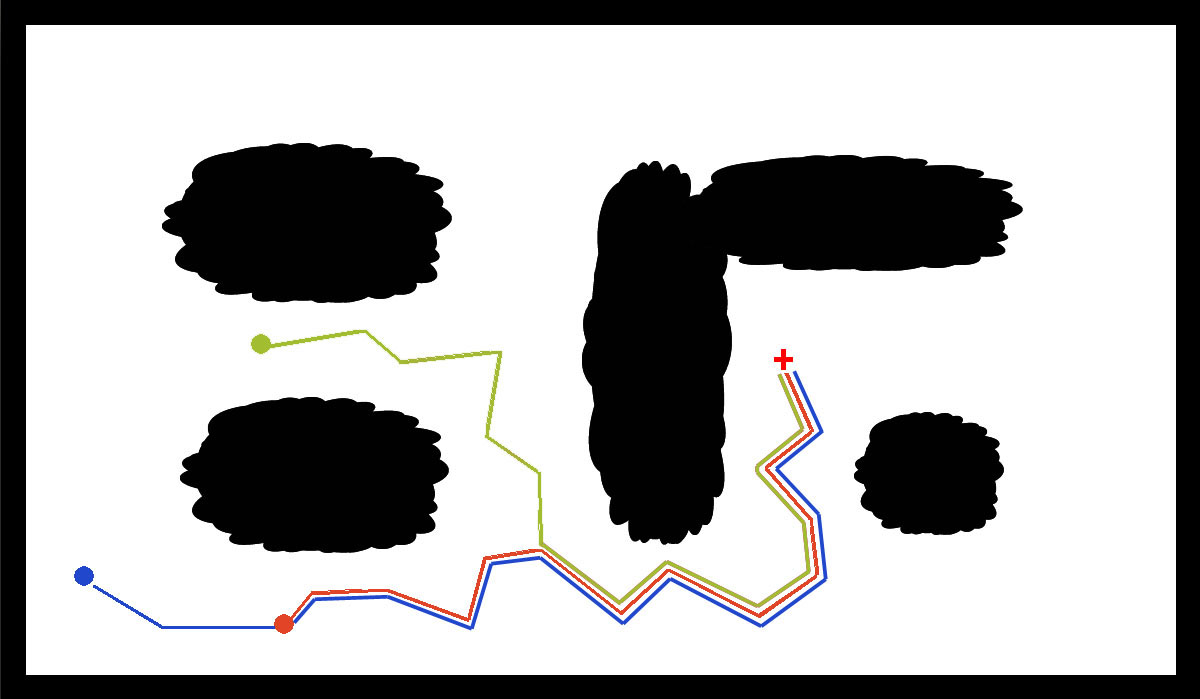
\includegraphics[width=0.25\textwidth]{figures/astar_contrast.jpg}
\hspace*{0.25cm}
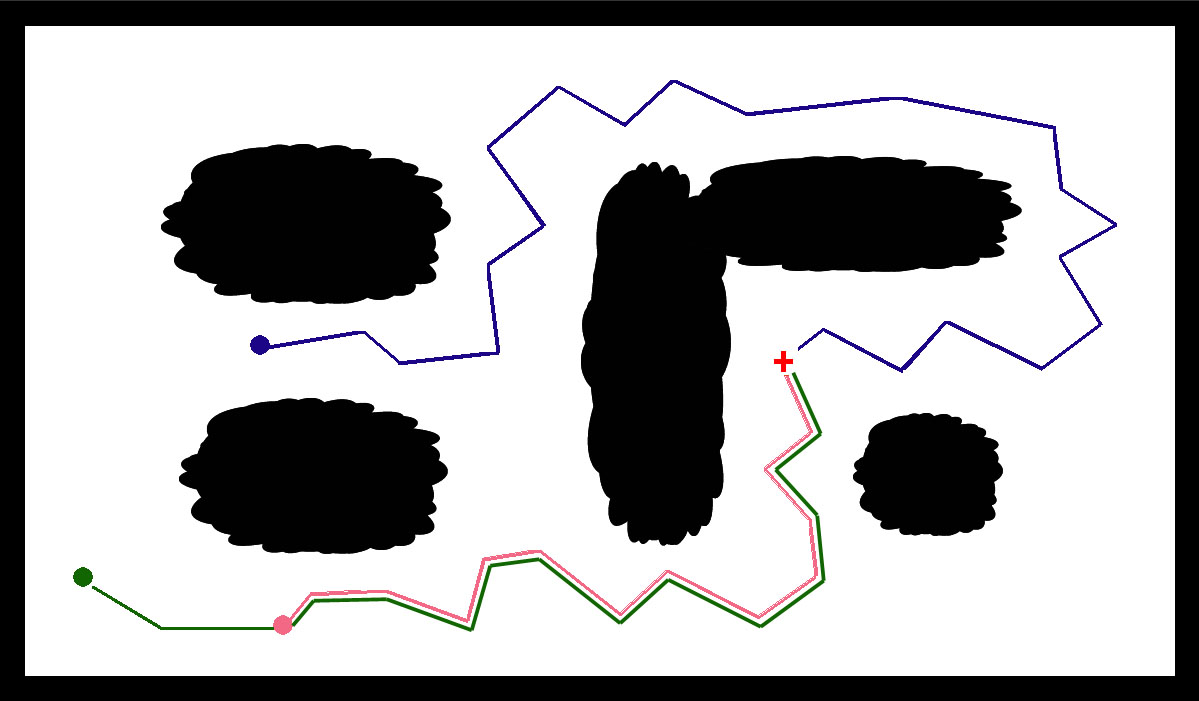
\includegraphics[width=0.25\textwidth]{figures/ambush_contrast.jpg}
\end{center}

\section*{A$^*$mbush Variations}

\begin{multicols}{3}
\begin{minipage}{0.3\textwidth}
\section*{P-A*mbush}

\begin{itemize}
\item If agent $i$ is the closest one to the goal, it
could be beneficial to make $i$ perform the path computing
first.

\item P-A$^*$ambush incorporates a strategy that decides
which agent calculates its path first.

\item We propose the real distance as a good strategy, because
the positions of the agents are a very general and intuitive
property that defines the advantage of an agent over another
one.

\end{itemize}

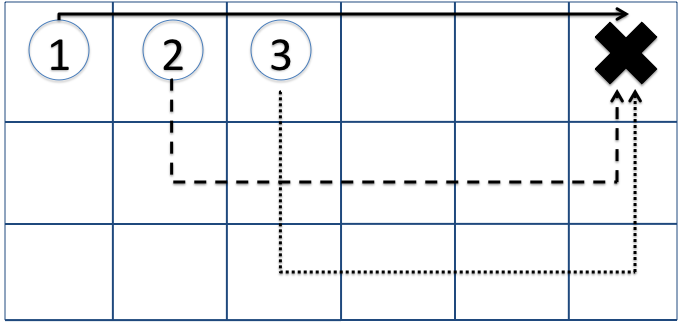
\includegraphics[width=0.48\textwidth]{figures/ambush_grid.png}
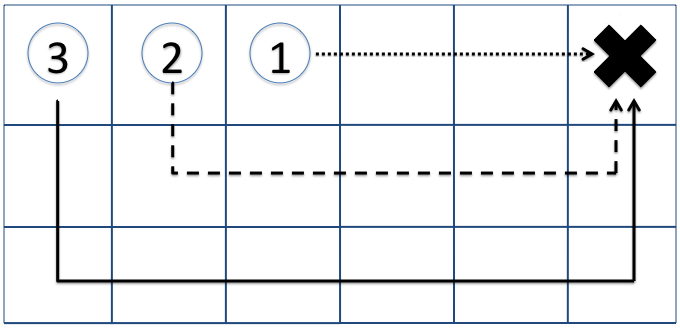
\includegraphics[width=0.48\textwidth]{figures/priorities_grid.png}
\end{minipage}

\documentclass[runningheads,a4paper]{llncs}

\usepackage{graphicx,times,amsmath, fontenc}
\usepackage{amssymb}
\usepackage{amsmath}
\newcommand{\bigO}{\mathcal{O}}
\newcommand{\astar}{$\textit{A}^*$ }
\newcommand{\ambush}{$\textit{A}^*\textit{mbush}$}
\newcommand{\rambush}{$\textit{R-}A^*\textit{ambush}$}
\newcommand{\sarambush}{$\textit{Self Adaptive R-}A^*\textit{ambush}$}
\setcounter{tocdepth}{3}
\usepackage{graphicx}

\usepackage{url}
\urldef{\mailsa}\path|{kelwin, glebys}@gia.usb.ve|
\urldef{\mailsc}\path|cchang@.usb.ve|    
\newcommand{\keywords}[1]{\par\addvspace\baselineskip
\noindent\keywordname\enspace\ignorespaces#1}

\begin{document}

\mainmatter  % start of an individual contribution

% first the title is needed
\title{A$^*$mbush, R-A$^*$mbush and Self Adaptive R-A$^*$mbush:
A$^*$ Variations for Ambush Behaviour And Path Diversity
Generation}

% a short form should be given in case it is too long for the running head
\titlerunning{A$^*$mbush, R-A$^*$mbush and Self Adaptive R-A$^*$mbush}

% the name(s) of the author(s) follow(s) next
%
% NB: Chinese authors should write their first names(s) in front of
% their surnames. This ensures that the names appear correctly in
% the running heads and the author index.
%
\author{Kelwin Fernandez \and Glebys Gonzalez \and Carolina Chang}
%
\authorrunning{A$^*$mbush, R-A$^*$mbush and Self Adaptive R-A$^*$mbush}
% (feature abused for this document to repeat the title also on left hand pages)

% the affiliations are given next; don't give your e-mail address
% unless you accept that it will be published
\institute{Grupo de Inteligencia Artificial,\\
Departamento de Computaci\'{o}n y Tecnolog\'{i}a de la Informaci\'{o}n\\
Universidad Sim\'{o}n Bol\'{i}var, Venezuela\\
\mailsa\\
\mailsc\\
\url{http://www.gia.usb.ve}}

%
% NB: a more complex sample for affiliations and the mapping to the
% corresponding authors can be found in the file "llncs.dem"
% (search for the string "\mainmatter" where a contribution starts).
% "llncs.dem" accompanies the document class "llncs.cls".
%

\toctitle{A$^*$mbush, R-A$^*$mbush and Self Adaptive R-A$^*$mbush}
\tocauthor{Fernandez, K. Gonzalez, G. Chang, C}
\maketitle


\begin{abstract}
A* is a commonly proposed algorithm 
for pathfinding in the area of Artificial Intelligence for
Videogames. Non playing characters use this algorithm often for
chasing others characters.
Even though A* guaranties optimality, it tends to bring forth
 similar behaviours in agents that are close to each other. On the other hand, 
when the agents are sparsely distributed, the algorithm doesn't secure
ambushes. We propose three algorithms for generating of ambush behaviors 
and diversity of paths: A*mbush, R-A*mbush and Self Adaptive
R-A$^*$mbush algorithms. They are
variations of A* that take into account the number of agents that have
a specific node (or edge)  in their calculated path. Additionally, R-A*mbush and Self Adaptive R-A$^*$mbush include strategies to minimize the
cost of the generated paths.
\end{abstract}

%------------------------------------------------------------------------
\section{Introducci\'on}

En el \'area de Inteligencia Artificial para Videojuegos, la generaci\'on
de conductas inteligentes ha sido un reto constante \cite{MF09}, frecuentemente
derivado en el desarrollo de acciones prestablecidas que el usuario puede
f\'acilmente identificar despu\'es de varias ejecuciones del juego.
Esta caracter\'istica es a\'un m\'as com\'un cuando se trata de la generaci\'on
de movimientos t\'acticos y estrat\'egicos grupales, los cuales suelen ser sumamente
complejos de implementar.

Un problema muy tratado en la literatura es la b\'usqueda de caminos
a un punto com\'un, por parte de grupos de agentes dentro de un juego
\cite{MF09}. Este punto suele venir dado por un lugar en el mapa de juego,
potencialmente la posici\'on del oponente. El esquema regularmente utilizado
es generar caminos de costo m\'inimo \cite{HNR72} \cite{RN93}
hacia este punto, sobre el grafo inducido por el mapa del juego. Es
muy probable, que estos caminos confluyan, evitando la diversidad de
rutas y exploraci\'on del mapa.

Al efectuar una persecuci\'on al oponente, la utilizaci\'on de caminos
\'optimos como estrategia deja muchos espacios de escapatoria libres,
por lo que es de especial inter\'es generar mecanismos de diversificaci\'on de
rutas que generen situaciones de emboscada.

\textbf{
En este punto hablar de nuestra soluci\'on y de como esta prob\'o ser
correcta. Mencionar que este art\'iculo pretende ser un soporte adicional
a los dos anteriores para demostrar la validez de las distintas variantes
de forma exhaustiva as\'i como tambi\'en de presentar una nueva m\'etrica
que permite medir de forma m\'as refinada el grado de emboscada.
}

\begin{comment}
La t\'ecnica expuesta pr\'oximamente es adaptable a muchos contextos en
los que, si bien no es necesaria una situaci\'on de emboscada, es
importante generar diversidad de caminos con el fin de no sobresaturar
ciertos sectores del grafo subyacente. Ejemplo de estos son controladores
de tr\'afico, enrutamiento de paquetes f\'isicos o digitales \cite{TMSV03},
rob\'otica, entre otros.
\end{comment}
\begin{minipage}{0.3\textwidth}

\section*{Formal Problem Definition}
\begin{itemize}
\item Let $G = (V,E)$ be a \textbf{graph} (directed or undirected).

\item Let $A$ be a \textbf{set of agents} that want to reach a point
$t \in V$. Every agent $i \in A$, is located in a node of the
graph. Let $pos(i)$ be the position of the agent $i$.

\item A function over $i$ is defined for  determining the
\textbf{cost} of the displacement of the agents  through the graph
$\lambda_i : E \longrightarrow \mathbb{R}^{\geq 0}$.

\item Let $path(i)$ having $i \in A$, be the \textbf{path} that the 
agent $i$ is taking to reach node $t$.

\item The \textbf{degree of ambush} towards the node $t$ is defined as:\\

$\Phi(t) = \dfrac{|\{ i : path(j) = <pos(j),\ \ldots,\ i,\ t>, j \in A\}|}
{\min(|\{ <i,t> : <i,t> \in E \} |,|A|) }$

\end{itemize}
\end{minipage}
%\section{A*}

The \astar algorithm \cite{art2,book4,book3} is a variation
of Dijkstra's algorithm \cite{book1} that computes 
paths of minimal cost.
It is an informed search algorithm \cite{book4}, based on 
the following elements:

\begin{itemize}
\item $g$: Represents the accumulated cost from the initial node to the actual node $v$.
\item $\hat{h}$: Is an estimate of the cost from the actual node $v$ to the goal.
\item $\hat{f} = g + \hat{h}$: An estimate of the cost from the initial node to the goal, having $v$ in the path..
\end{itemize}

For the sake of securing optimality, the $\hat{h}$ heuristic 
must be admissible, that is, it shouldn't overestimate any 
cost against the optimal solution.
This algorithm works in a greedy fashion, expanding the next unexplored 
node with the smallest estimated cost $\hat{f}$ at the moment. 
This procedure is repeated until the goal is reached. 

% fin de la nueva def y luego viene lo del orden del algoritmo

The estimated running time of $A^*$ is
$\bigO(|V|log(|V|) + |V|*h + |E|)$.
Having $h$ as the cost of computing function
$\hat{h}$. This cost is derived, assuming an
efficient implementation of the priority queue
such as a Fibonacci heap \cite{book1} and that
the heuristic of each node is only computed
once.
\section{A*mbush}

In this section we propose \ambush, an $A^*$-based
algorithm that solves the ambush generation problem. 
It consists in a modification of $g$ function, that favours
path diversity. We will call this function $g'$.

Let $\Psi(v,i) = 1+(\# j : j \in A \wedge v \in path(j))$,
be the number of agents different from agent $i$, that have the 
node $v$ in their paths towards $t$ plus one. If an agent is not trying to 
reach node $t$ at the moment, or it has not performed the 
search for the node yet, it's path counts as empty. 
Therefore, the agent is not taken into account when calculating
$\Psi(v,i)$'s value. 

It is considered that $g'(pos(i),i) = 0$ for the initial node.
 Let $<v,w>$ be the next edge that should be expanded
from the node $v$, in any of the algorithm's iterations. In
these conditions, the expression that determines $g'$'s value
is $g'(w, i) = g'(v,i) + \lambda_i(<v,w>) \cdot \Psi(w,i)^2$.

Given that $\Psi(v,i) \geq 1$, the path determined by $A^*mbush$
is optimal under the new definition of $g'$. Hence, the properties of
 $A^*$ are preserved \cite{art2}. Nevertheless the path might not 
 be optimal for the original costs function $g$.

Note that $\Psi(v,i) = 1$ for every node $v$ that is not considered
in the path of any agent different to $i$. Similarly,
$\Psi(v,i) > 1$ in any other case. This condition allows the 
agents to consider exploring sub-optimal paths in the 
original graph. The less agents explore this routes, the greater
the chance given to other agents to travel trough them.

\subsection{Complexity}

It is possible to precompute the
function $\Psi$ for node cost's increment. If this function is stored
in a constant structure with fast access, the cost of calculating
$g'$ becomes equal to the cost of computing $g$.
Therefore, the only change if the algorithm's cost
 lays in the initial calculation of function $\Psi$.

The asymptotic complexity of $A^*mbush$ is:
$\bigO(|V|log(|V|) + |V|*h + |E| + |A|*|V| )$.

In the field of video games, the graphs of interest are
given by the polygonal division scheme of the map
\cite{book3,art1} (this polygons tend to have a small
amount of sides), according to the traversable regions 
and their respective adjacencies \cite{book3,art1}. 
Since the number of sides for the polygons is small, this 
graphs tend to have little density. In consequence,
$|E| \in \bigO(|V|)$, this means that the execution 
time of this methods for the graphs of interest in the
area of video games, is considered to be
$\bigO(|V|(log(|V|) + h + |A|) )$. 
The amortized cost of the increment function is $\bigO(|V|)$,
therefore, the amortized cost of the A$^*$mbush algorithm
equals the A$^*$ cost.

\begin{comment}
Figure
\ref{fig:graph_decomp} shows a clear example of a map 
broken into polygons. Each one of them is considered to
be a node in the search space. Two nodes are adjacent if 
their polygons share a common side. 

\begin{figure}[htp]
\centerline{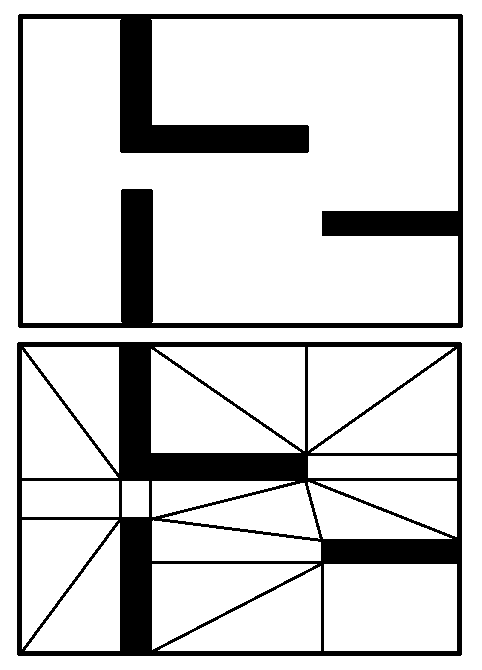
\includegraphics[width=0.6\columnwidth]{figures/graph_decomposition.png}}
\caption{Up: Game map, the black blocks are the obstacles
              Down: Decomposition of the map into convex polygons}
\label{fig:graph_decomp}
\end{figure}
\end{comment}


\section{ R-A*mbush: Ambush with fixed radio R}

Getting agents to perform \ambush\ from the starting 
point can be disadvantageous, since they can take 
unnecessarily longer routes, when avoiding each other’s paths. 
Making the agents perform \ambush\ when they are closer
 to the goal could shorten the increment in this cost. 
 
With this reasoning as a base, \rambush\ is proposed.
 It is an A$^*$mbush modification that performs \astar until
the agent gets inside a fixed radius $R$ around the goal point.
Once at this stage, the agent stats performing \ambush. 
Note that this transition happens only once. Even if  the
\ambush\ algorithm makes the agent leave the radio area,
it will not start performing \astar again. This prevents a 
loop that the intelligence could easily fall into. First, the agent,
following the path given by A$^*$ comes inside the radius R,
then \ambush\ takes it out of the area when trying to go for 
a unexplored route, subsequently, this behaviour is interrupted 
and the A$^*$ method takes control again, making the agent go 
inside the radio. Those steps could be repeated infinitely, 
so once the radio $R$ is crossed, only \ambush\ behaviour takes place.
Figure \ref{fig:rambush} shows the performance of the \rambush\
algorithm.

\begin{figure}[htb]
	\centerline{
		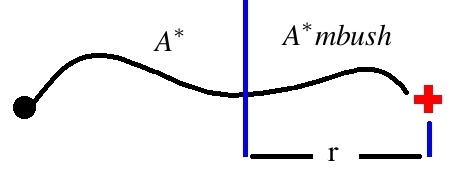
\includegraphics[width=0.48\columnwidth]{figures/rambush.jpg}
	}
	\caption{\label{fig:rambush}
	     R-A$^*$mbush. The agent located in the black point
	     tries to reach the cross.}
\end{figure}

The radius $R$ is measured in real distance (A$^*$). 
It was chosen over the Euclidean, because obstacles in games 
could make the agents take ambush routes when the path to 
get to the goal is still very long, and this would antagonize 
the purpose of reducing the path cost when possible.

\section{ Self Adaptive R-A*mbush: Ambush with adaptive radius R}

\rambush\  provides a solution that is not as general as the one for
 \ambush.  Using the same distance $R$ for the fixed radius 
 in different maps, would produce good results in some of them 
 and bad ones in others. This means the user would have to manually 
 fix the measure of $R$ by tacking into consideration the size of 
 the map, the path cost function, or the number of obstacles. 
 In addition, given that  the cost function can be different for each 
 agent, the radius should be established according to the 
 $\lambda$ measure of every agent.
  
Thus, \sarambush\ is proposed as a variation of \rambush\ that 
solves this generality problem. Initially, This method makes each
 agent calculate the path with \astar. Then, a set of points from
  that route is chosen.  This will  be the set of the possible radius 
  $R$. The algorithm will select the minimum radius that generates 
  the greatest $\Phi$, starting from the smallest $R$.  
  This is based on the idea of starting to use sub-optimal 
  paths as late as possible.  Note that \astar\ is the specific 
  case where $R=0$ and \ambush\ is the one where $R$ is greater 
  than or equal to the real distance between the agent and the goal.  

If points that are too close to the goal are inside the set of radius, 
in particular, $R=0$, all the other agents will choose the optimal path, 
once the maximum ambush is reached. This could make the 
distribution of the agents around the goal very unbalanced towards 
the nodes that are closest to the agents stating points.

Figure \ref{unbalanced} Shows a situation where the agents distribution 
is not desirable, but the maximum ambush rate is obtained.	The agents 
colored in black performed the method \sarambush\ first. Then, the agents
in gray chose the optimal path because the ambush measure cannot 
be improved anymore, creating an unbalanced distribution around the
goal. This can be solved by taking into account a measure
 of distribution when choosing the radius. Thus, let 

\begin{equation}
  \Delta = 1-\dfrac{(\Sigma i |  i \in V 
  						\wedge i \in pred(t)
  						\wedge num(i) > 
  							\left\lceil \frac{n}{|pred(t)|} \right\rceil 
  					:  num(i) - 
  						\left\lceil \frac{n}{|pred(t)|} \right\rceil}		
  						{n-\left\lfloor \frac{n}{|pred(t)|} \right\rfloor}
\end{equation}

\noindent
be a metric related with the rate of agents that need to
reach the goal from another node to have them equally
distributed. The value of the metric is 1 when the
agents are perfectly distributed and it tends to zero
when the agents are unbalanced.
In the formula, $n$ represents the number of agents that
already calculated the path.  $pred(t)$  is the set of nodes adjacent to
the goal node. Finally $num(i)$ is the number of agents that reached 
the target from the node $i$. 
The numerator of the main fraction counts the number of the agents
that need to be swapped and the denominator is the number of
swaps in the worst case scenario (all agents reaching the goal
from one node). The only purpose of the subtraction is to
use the lexicographical order in the objective function of
the strategy.
For example, for Figure \ref{unbalanced} $\Delta = 0.66$.
This means that equal distribution can be reached by making one of
the agents that are on the node at the left of the goal, ambush it
from above.

\begin{figure}[htb]
	\centerline{
		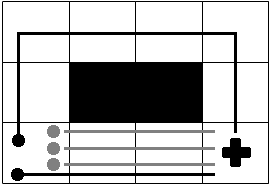
\includegraphics[width=0.48\columnwidth]{figures/unbalanced.png}
	}
	\caption{\label{unbalanced}
	     Unbalanced ambush.}
\end{figure}

The algorithm would search for the maximum ambush
rate and in case of a tie it would go for the path that
achieves the best distribution. The $\Delta$ value alone is
not enough to compare two ambush strategies.

\subsection{Complexity}

This variation of \ambush\ is more inefficient than the
original version. If $T(G,A)$ is the
complexity in time of computing \ambush\ for a graph
$G=(V,E)$ with $|A|$ agents and the number of candidates 
to be selected as radius points is $k$, the complexity
of the \sarambush\ is $\bigO(k\cdot T(G,A))$.

Since $k \in \bigO(V)$ (selecting every possible node
as radius) the worst case of the algorithm is
$\bigO(|V|\cdot T(G,A))$. Alternative candidate sets
can be constructed from taking nodes that are separated
by distances that are incremented exponentially, for
example, selecting the nodes in positions that are
powers of two in the \astar\ path ($1, 2, 4, 8, \ldots$).
This variation leads to an increment of only $\bigO(log(|V|))$.
In the following experiments the radius set contains
every node in the \astar\ path.

\section{Experimentos}
\label{sec:experiments}

Para cada experimento se estudian cinco algoritmos:
una implementaci\'on base de \astar que sirve de referencia,
una implementaci\'on de caminos simples aleatorios mediante
b\'usqueda en profundidad, \ambush, \pambush con mecanismo
de prioridad determinado por la distancia real de los agentes
a la meta y finalmente, \sarambush.

presentan resultados del incremento medio porcentual de los caminos.
Para cada topolog\'ia de grafo, se generan aleatoriamente 100 grafos,
sobre los cuales se ejecutan experimentos con 100 disposiciones distintas
de agentes y del nodo objetivo.
Para cada uno de estos algoritmos se muestra el valor de emboscada
utilizando la m\'etrica originalmente propuesta y utilizando la
m\'etrica propuesta en el presente trabajo. El n\'umero de agentes
es variado con el fin de mostrar su impacto en el grado de emboscada
y en el incremento derivado de la escogencia de caminos sub\'optimos.
Adem\'as se muestran resultados con las dos instancias de mapas ($g1$ y $g2$)
presentadas en el trabajo previo \cite{FGC12} con 60 y 85 nodos
respectivamente. Estos mapas provienen de la poligonalizaci\'on del mapa
de juego en pol\'igonos. Estas restricciones son ampliamente utilizadas
en juegos\cite{MF09}. Estos grafos se pueden visualizar en la figura \ref{fig:gs}.

\begin{figure}[htb]
	\begin{center}
		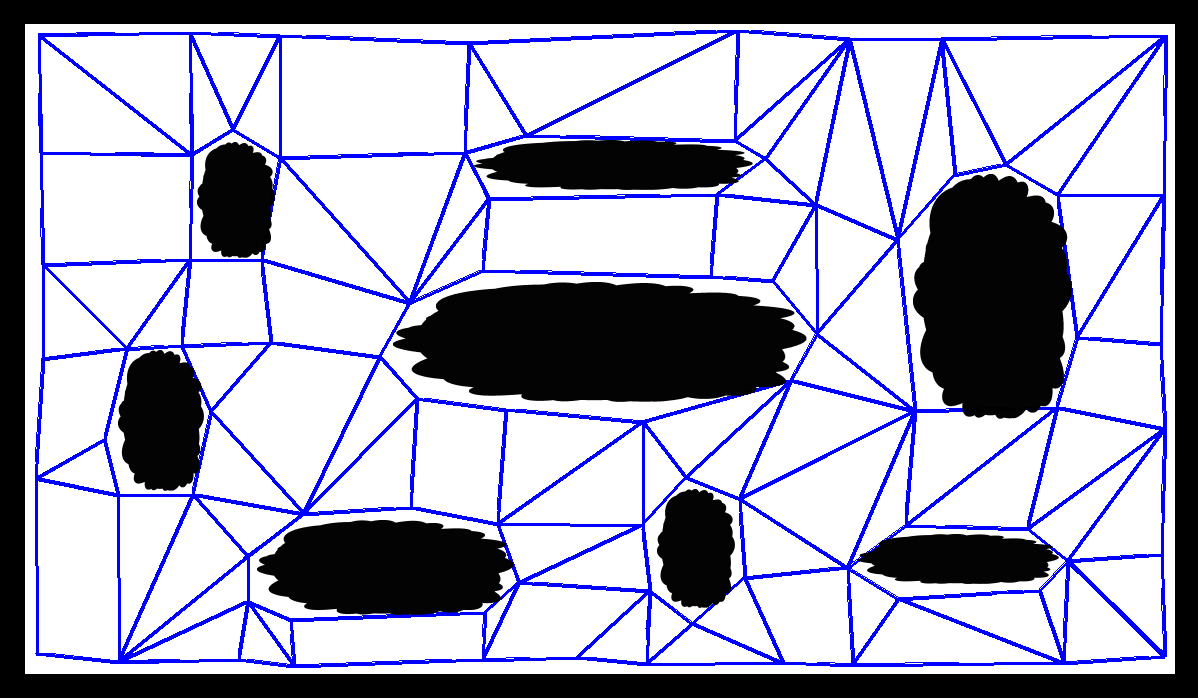
\includegraphics[scale=0.23]{figures/g1.png}
		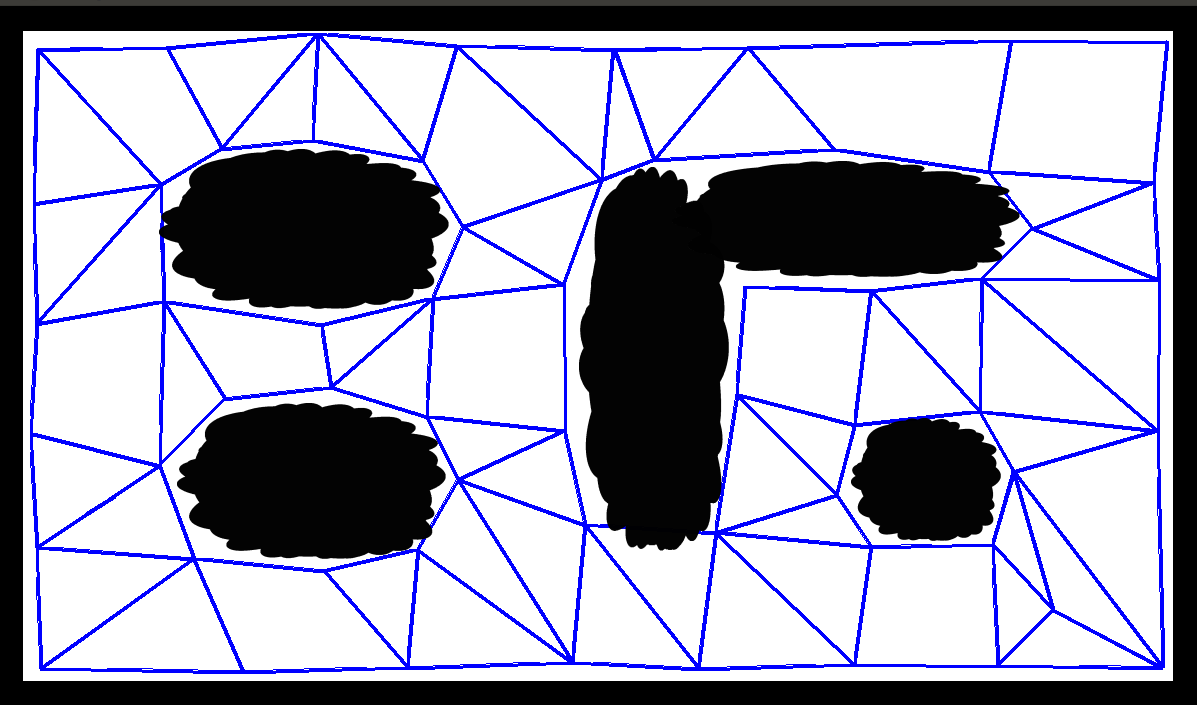
\includegraphics[scale=0.23]{figures/g2.png}
	\end{center}
	\caption{\label{fig:gs}
	     \textbf{Arriba:} Mapa 1 poligonalizado (60 pol\'igonos).
	     \textbf{Abajo:} Mapa 2 poligonalizado (85 pol\'igonos).
     }
\end{figure}


\end{document}
\section{Cosas del formato que es mejor no borrar aun}

Displayed equations or formulas are centered and set on a separate
line (with an extra line or halfline space above and below). Displayed
expressions should be numbered for reference. The numbers should be
consecutive within each section or within the contribution,
with numbers enclosed in parentheses and set on the right margin --
which is the default if you use the \emph{equation} environment, e.g.,
\begin{equation}
  \psi (u) = \int_{o}^{T} \left[\frac{1}{2}
  \left(\Lambda_{o}^{-1} u,u\right) + N^{\ast} (-u)\right] dt \;  .
\end{equation}

Equations should be punctuated in the same way as ordinary
text but with a small space before the end punctuation mark.


\begin{figure}
\centering
%\includegraphics[height=6.2cm]{eijkel2}
\caption{One kernel at $x_s$ (\emph{dotted kernel}) or two kernels at
$x_i$ and $x_j$ (\textit{left and right}) lead to the same summed estimate
at $x_s$. This shows a figure consisting of different types of
lines. Elements of the figure described in the caption should be set in
italics, in parentheses, as shown in this sample caption.}
\label{fig:example}
\end{figure}

\subsection{Program Code}

Program listings or program commands in the text are normally set in
typewriter font, e.g., CMTT10 or Courier.

\medskip

\noindent
{\it Example of a Computer Program}
\begin{verbatim}
blabla el codigo
\end{verbatim}
%
\noindent
{\small (Example from Jensen K., Wirth N. (1991) Pascal user manual and
report. Springer, New York)}

\subsection{Citations}

For citations in the text please use
square brackets and consecutive numbers: \cite{jour}, \cite{lncschap},
\cite{proceeding1} -- provided automatically
by \LaTeX 's \verb|\cite| \dots\verb|\bibitem| mechanism.

\begin{thebibliography}{4}

\bibitem{book1}
T.~Cormen, C.~Leiserson, R.~Rivest and C. Stein, \emph{Introduction to Algorithms, 3rd ed}.\hskip 1em plus 0.5em minus 0.4em\relax
  The MIT Press, 2009.
  
\bibitem{book2}
M.~Gendreau and J.~Potvin, \emph{Handbook of Metaheuristics, 2nd ed}.\hskip 1em plus 0.5em minus 0.4em\relax
  Springer, 2010.  

\bibitem{book3}
I.~Millington and J.~Funge, \emph{Artificial Intelligence for Games, 2nd ed}.\hskip 1em plus 0.5em minus 0.4em\relax
  Morgan Kaufmann Publishers, 2009.  

\bibitem{book4}
S.~Russell and P.~Norvig, \emph{Artificial Intelligence: A Modern Approach, 2nd ed}.\hskip 1em plus 0.5em minus 0.4em\relax
  	Prentice-Hall, Englewood Cliffs, NJ,, 1993.  
  
\bibitem{art1}
X.~Cui and H.~Shii, ``Direction oriented pathfinding in video games,'' \emph{International Journal of Artificial Intelligence  \& applications 2}, 2011.

\bibitem{art2}
P.~Hart, N.~Nilsson and B.~Raphael, ``Correction to “a formal basis for the heuristic determination of minimum cost paths”,'' \emph{SIGART Newsletter 37}, pp. 28--29, 1972.

\bibitem{art3}
D.~Silver, ``Cooperative pathfinding,'' \emph{ AI Game Programming Wisdom 3}, pp. 99--111, 2006.

\bibitem{art4}
R.~Teixeira, K.~Marzullo, S.~Savaje and G.~Voelker, ``In search of path diversity in isp networks,'' \emph{ IMC}, pp. 27--29, 2003.

\bibitem{web1}
E.~Haines, ``Point in Polygon Strategies,''
\emph{http://erich.realtimerendering.com/ ptinpoly/}, 2001.

\bibitem{BRO89}
A. Broder, `` Generating random spanning trees''. In \emph{Proceedings of the 30th IEEE Symposium
on Foundations of Computer Science}, pp 442--447, 1989.

\bibitem{jour} Smith, T.F., Waterman, M.S.: Identification of Common Molecular
Subsequences. J. Mol. Biol. 147, 195--197 (1981)

\bibitem{lncschap} May, P., Ehrlich, H.C., Steinke, T.: ZIB Structure Prediction Pipeline:
Composing a Complex Biological Workflow through Web Services. In: Nagel,
W.E., Walter, W.V., Lehner, W. (eds.) Euro-Par 2006. LNCS, vol. 4128,
pp. 1148--1158. Springer, Heidelberg (2006)

\bibitem{book} Foster, I., Kesselman, C.: The Grid: Blueprint for a New Computing
Infrastructure. Morgan Kaufmann, San Francisco (1999)

\bibitem{proceeding1} Czajkowski, K., Fitzgerald, S., Foster, I., Kesselman, C.: Grid
Information Services for Distributed Resource Sharing. In: 10th IEEE
International Symposium on High Performance Distributed Computing, pp.
181--184. IEEE Press, New York (2001)

\bibitem{proceeding2} Foster, I., Kesselman, C., Nick, J., Tuecke, S.: The Physiology of the
Grid: an Open Grid Services Architecture for Distributed Systems
Integration. Technical report, Global Grid Forum (2002)

\bibitem{url} National Center for Biotechnology Information, \url{http://www.ncbi.nlm.nih.gov}

\end{thebibliography}



\end{document}

\begin{minipage}{0.3\textwidth}
\section*{SAR-A*mbush}

\begin{itemize}
\item Using the same distance R for the fixed radius in
different maps, would produce good results in some of them
and bad ones in others. This means the user would have to
\textbf{manually fix} the measure of R.

\item We propose SAR-A$^∗$mbush as a variation of
R-A$^∗$ambush.

\item Initially, this method makes each agent calculate the
path with A$^∗$. Then, a \textbf{set of points} from that route is chosen.
This will be the set of the possible radius R.

\item The algorithm will select the \textbf{minimum radius} that
generates the \textbf{greatest} $\Phi$, starting
from the smallest R.

\item In case of a \textbf{tie in the maximum ambush} value, it would go
for the path that achieves the \textbf{best distribution} of the agents.

\end{itemize}
\end{minipage}
\end{multicols}

\section*{Experiments}
\begin{multicols}{2}
\begin{table}[h]
\caption{Ambush rate ($\Phi$) - 2-100 agents}
\begin{center}

\begin{tabular}{|c|c|c|c|c|c||c|c|c|c|c|c|c|}
\hline
 & 
\multicolumn{5}{|c||}{\textbf{Map 1 (60 nodes)}} &
\multicolumn{5}{|c|}{\textbf{Map 2 (85 nodes)}}\\
\hline
\# & $A^*$ & $RST$ & $A^*mbush$ & $P$ & $SAR$ &
	 $A^*$ & $RST$ & $A^*mbush$ & $P$ & $SAR$\\
\hline
 2 & 0.72 & 0.75 & 0.87 & \textbf{0.89} & 0.87 &
	 0.72 & 0.75 & 0.88 & \textbf{0.91} & 0.89\\
% 3 & 0.79 & 0.83 & 0.95 & \textbf{0.96} & 0.95 &
%	 0.76 & 0.82 & 0.95 & \textbf{0.96} & \textbf{0.96}\\
 4 & 0.85 & 0.90 & 0.98 & \textbf{0.99} & 0.98 &
	 0.83 & 0.88 & 0.98 & \textbf{0.99} & 0.98\\
% 5 & 0.89 & 0.93 & \textbf{0.99} & \textbf{0.99} & \textbf{0.99} &
%	 0.87 & 0.92 & 0.99 & 0.99 & \textbf{1.00}\\
 6 & 0.91 & 0.96 & \textbf{0.99} & \textbf{0.99} & \textbf{0.99} &
	 0.90 & 0.95 & \textbf{1.00} & 0.99 & \textbf{1.00}\\
 8 & 0.95 & 0.98 & \textbf{0.99} & \textbf{0.99} & \textbf{0.99} &
	0.93 & 0.97 & \textbf{1.00} & \textbf{1.00} & \textbf{1.00}\\
10 & 0.96 & 0.99 & \textbf{1.00} & \textbf{1.00} & \textbf{1.00} &
	 0.95 & 0.99 & \textbf{1.00} & \textbf{1.00} & \textbf{1.00}\\
%15 & 0.98 & 0.99 & \textbf{1.00} & \textbf{1.00} & \textbf{1.00} &
%	 0.98 & \textbf{1.00} & \textbf{1.00} & \textbf{1.00} & \textbf{1.00}\\
20 & 0.99 & \textbf{1.00} & \textbf{1.00} & \textbf{1.00} & \textbf{1.00} &
     0.99 & \textbf{1.00} & \textbf{1.00} & \textbf{1.00} & \textbf{1.00}\\
50 & 0.99 & \textbf{1.00} & \textbf{1.00} & \textbf{1.00} & \textbf{1.00} &
	\textbf{1.00} & \textbf{1.00} & \textbf{1.00} & \textbf{1.00} & 
	\textbf{1.00}\\
75 & 0.99 & \textbf{1.00} & \textbf{1.00} & \textbf{1.00} & \textbf{1.00} &
	\textbf{1.00} & \textbf{1.00} & \textbf{1.00} & \textbf{1.00} &
	\textbf{1.00}\\
100 & \textbf{1.00} & \textbf{1.00} & \textbf{1.00} & \textbf{1.00} & 
	\textbf{1.00} & 
	\textbf{1.00} & \textbf{1.00} & \textbf{1.00} & \textbf{1.00} & \textbf{1.00}\\
\hline
\end{tabular}

\label{ambushrate}
\end{center}
\end{table}
\begin{table}

\caption{$\Phi$ and Mean of the Incremental Distance 
		 with Multiscale Graphs (6 agents)}
\begin{center}

\begin{tabular}{|c|c|c|c|c|c||c|c|c|c|c|}
\hline
& \multicolumn{5}{|c||}{\textbf{Ambush Rate}} &
  \multicolumn{4}{|c|}{\textbf{Incremental Distance}}\\
\hline
  $Nodes$ & $A^*$ & $RST$ & $A^*mbush$ & $P$ & $SAR$
		  		  & $RST$ & $A^*mbush$ & $P$ & $SAR$\\
\hline
   85 & 0.88 & 0.97 & \textbf{1.00} & \textbf{1.00} & \textbf{1.00}
      & 83.05 & 20.12 & 22.30 & \textbf{13.99}\\
  170 & 0.92 & 0.97 & \textbf{1.00} & 0.99 & \textbf{1.00}
	  & 90.06 & 20.34 & 17.89 & \textbf{12.22}\\
  425 & 0.78 & 0.94 & 0.97 & \textbf{0.98} & \textbf{0.98}
	  & 101.17 & 23.06 & 17.07 & \textbf{11.44}\\
  850 & 0.80 & 0.94 & 0.96 & \textbf{0.97} & \textbf{0.97}
	  & 130.80 & 16.86 & 11.66 & \textbf{6.13}\\
 1700 & 0.76 & 0.94 & \textbf{1.00} & 0.97 & \textbf{1.00}
	  & 119.47 & 9.28 & \textbf{5.35} & 5.96\\
\hline
\end{tabular}

\label{tab:multiscale}
\end{center}
\end{table}

\section*{Computational Complexity ($\bigO$)}

\begin{center}
A$^*$ $=$ A$^*$mbush, R$^*$mbush $\leq$ P-A$^*$mbush
$\leq$ SAR-A$^*$mbush
\end{center}
\end{multicols}
\end{document}

